%% chapters/chapter_1.tex
%%
%% Copyright 2017 Evandro Coan
%% Copyright 2012-2014 by abnTeX2 group at http://abntex2.googlecode.com/
%%
%% This work may be distributed and/or modified under the
%% conditions of the LaTeX Project Public License, either version 1.3
%% of this license or (at your option) any later version.
%% The latest version of this license is in
%%   http://www.latex-project.org/lppl.txt
%% and version 1.3 or later is part of all distributions of LaTeX
%% version 2005/12/01 or later.
%%
%% This work has the LPPL maintenance status `maintained'.
%%
%% The Current Maintainer of this work is the Evandro Coan.
%%
%% The last Maintainer of this work was the abnTeX2 team, led
%% by Lauro César Araujo. Further information are available on
%% https://www.abntex.net.br/
%%
%% This work consists of a bunch of files. But originally there were 2 files
%% which are renamed as follows:
%% Deleted the `abntex2-modelo-img-marca.pdf`
%% Renamed the `abntex2-modelo-include-comandos.tex, v-1.9.2 laurocesar` to `chapters/chapter_1.tex`
%%
% ---
% Este capítulo, utilizado por diferentes exemplos do abnTeX2, ilustra o uso de
% comandos do abnTeX2 e de LaTeX.
% ---

% The \phantomsection command is needed to create a link to a place in the document that is not a
% figure, equation, table, section, subsection, chapter, etc.
%
% When do I need to invoke \phantomsection?
% https://tex.stackexchange.com/questions/44088/when-do-i-need-to-invoke-phantomsection
\phantomsection


% Is it possible to keep my translation together with original text?
% https://tex.stackexchange.com/questions/5076/is-it-possible-to-keep-my-translation-together-with-original-text
\chapter{Fundamentação Teórica}
\label{cap:fundamentacao_teorica}

% \newpage

Esta seção apresenta a fundamentação teórica sobre sistemas com múltiplos processadores, o processador \manycore \mppa, o padrão estêncil e o \fw \pskelmppa.

\section{Sistemas com múltiplos processadores}
\label{sec:multicpu}

\textit{Tanenbaum}~\cite{Tanenbaum:2014:MOS:2655363} classifica sistemas com múltiplos processadores em dois grupos, os sistemas multiprocessadores e os multicomputadores. Nesta seção serão apresentados os principais conceitos dos sistemas multiprocessadores e multicomputadores.

\subsection{Multiprocessadores}
\label{subsec:multiprocessadores}

O multiprocessador é um sistema de computadores no qual qual duas ou mais \textit{Central Processing Units} (\cpus) compartilham acesso total a uma \textit{Random Access Memory} (\ram). Assim, programas executando em qualquer uma das \cpus realizam operações de leitura e escrita em um espaço de endereçamento físico único na \ram. A particularidade que este sistema apresenta, é que ao escrever um valor na memória, posteriormente ao ler este mesmo valor ele pode obter um resultado diferente daquele que foi escrito, pois outra \cpu pode alterá-lo. Percebe-se que este comportamento pode causar inconsistências no sistema, e por isso é de extrema importância que recebam o tratamento adequado, que quando realizado, constitui a base para a comunicação entre processadores.

Apesar da propriedade de endereçamento total da memória, alguns multiprocessadores possuem a propriedade adicional de que cada palavra da memória pode ser lida tão rápido quanto a leitura de qualquer outra palavra presente na memória, essas máquinas são denominadas multiprocessadores com acesso uniforme à memória -- \textit{Uniform Memory Access} (\uma). Outrossim, existem os multiprocessadores com acesso não uniforme à memória -- \textit{Nonuniform Memory Access} (\numa).

\subsubsection{Multiprocessadores UMA}
\label{subsubsec:hw-multiprocessadores-uma}

Os multiprocessadores UMA possuem variações nas suas arquiteturas. Os mais simples são os baseados em barramento no qual o barramento é utilizado para comunicação, desta maneira, quando uma \cpu deseja ler uma palavra da memória, será verificada a disponibilidade do barramento, estando disponível a \cpu informa o endereço no barramento e junto de alguns sinais de controle aguarda até que a memória coloque a palavra requisitada no barramento. Porém, quando o barramento está indisponível a \cpu que deseja realizar leitura ou escrita da memória deve esperar até que o mesmo fique disponível. Quando existem poucas \cpus é possível realizar este gerenciamento, porém quando o número de \cpus aumenta surge o problema, pois o sistema passa a possuir um gargalo no barramento o que deixará muitas \cpus ociosas por muito tempo.

Uma maneira de reduzir o gargalo no barramento é através do uso de \textit{caches}, dessa maneira requisições satisfeitas pela \textit{cache} local não precisam ser realizadas através do barramento, desafogando o tráfego no mesmo e possibilitando o suporte a mais \cpus no sistema. Com o uso de \textit{caches} surge também a necessidade de estabelecer a coerência entre as \textit{caches} presente no sistema, e para isso são utilizados protocolos de coerência de \textit{cache} que serão responsáveis em manter a memória e as \textit{caches} em um estado consistente.

\subsubsection{Multiprocessadores NUMA}
\label{subsubsec:hw-multiprocessadores-numa}

Mesmo com o melhor sistema de \textit{cache}, o uso de um único barramento limita o tamanho de um multiprocessador UMA para cerca de 16 ou 32 \cpus \cite{Tanenbaum:2014:MOS:2655363}. Para aumentar o número de \cpus e necessário ir além, e utilizar arquiteturas como, barramento cruzado ou redes de comutação multi-estágio, porém estas arquiteturas necessitam de muito hardware, são caras, e não são tão maiores que as de barramento único. Para atingir a casa das dezenas de \cpus é necessário dispensar algo. E normalmente o que é dispensado é o tempo de acesso uniforme para todos os módulos de memória. Isso resulta na ideia de multiprocessadores NUMA. Assim como nos UMA, o espaço de endereçamento é único entre as \cpus, porém o tempo de acesso aos módulos de memória locais é mais rápido que o acesso aos módulos remotos.

Existem dois grupos entre os NUMA, os que fazem uso da coerência de \textit{cache} \textit{Cache-Coherent NUMA} (CC-NUMA) e os que não fazem \textit{Non Cache-coherent NUMA} (NC-NUMA). Os sistemas NUMA possuem nós compostos por \cpu, \textit{cache}, dispositivos de \io e estão conectados por uma rede de interconexão.

\subsubsection{\textit{Chips} multinúcleo (\multicore)}
\label{subsubsec:chips-multinucleo}

Os avanços tecnológicos na fabricação de chips resultam em transistores cada vez menores, possibilitando o uso de cada vez mais deles em um único \chip. Com tamanha quantidade de transistores em um único \chip é possível explorar os megabytes de \textit{cache} neles, porém existem limitações que fazem com que em um determinado ponto o aumento da \textit{cache} gere um ganho de apenas 0,5\% na taxa acerto. Desta maneira, outra possibilidade é colocar múltiplas \cpus completas, denominadas normalmente de núcleos, em um mesmo \chip. Já são comuns \chips com até 8 (oito) núcleos, e a presença de \textit{caches}, cruciais para o sistema, espalhadas pelo \chip.

\textit{Chips} multinúcleo são multiprocessadores muito pequenos, também são chamados de multiprocessadores em \chip~-- \textit{Chip MultiProcessors} (CMPs). Estes \chips são semelhantes aos multiprocessadores baseados em barramento ou redes de comunicação. O que os difere destes, é a fato das \cpus serem  conectadas muito próximas, assim falhas em componentes compartilhados podem acarretar na indisponibilidade de várias \cpus ao mesmo tempo, fato este que é improvável de ocorrer nos multiprocessadores tradicionais.

Também existem os sistemas em \chip~-- \textit{System on a Chip} (SoC), compostos de \cpus principais para processamento geral e de núcleos para tarefas específicas, como decodificação de aúdio e vídeo, criptoprocessadores, entre outros.

\subsubsection{\textit{Chips} com muitos núcleos (\manycore)}
\label{subsubsec:chips-manycore}

Os \manycore são \multicore que contêm dezenas, centenas ou até milhares de núcleos. Embora não exista uma delimitação clara de quando um \multicore torna-se um \manycore, uma analogia utilizada é que um \multicore é um \manycore a partir do momento que a perda de um ou dois núcleos seja irrelevante \cite{Tanenbaum:2014:MOS:2655363}.

A presença de um elevado número de núcleos em um mesmo \chip acarreta em impactos sobre a coerência de \textit{cache}, principalmente quanto ao custo e complexidade dos protocolos de coerência que atingem um limite a partir do qual ele passa a prejudicar o desempenho do sistema em questão. Devido a isso, processadores \textit{manycore} tendem a não utilizar \textit{caches} coerentes \cite{Tanenbaum:2014:MOS:2655363}.

A presença de milhares de núcleos não é algo mais tão incomum, as unidades de processamento gráfico -- \textit{Graphic Processing Unit} (\gpu), presente em muitos sistemas computacionais de hoje em dia, são detentores de milhares de pequenos núcleos com enfoque no processamento de dados, e realizam muito menos operações de coerência de \textit{cache} e lógicas de controle que as \cpus de propósito geral. Estas mudanças estão refletidas na maneira de se programar para esses sistemas, que a exemplos das \gpus utilizam linguagens específicas de programação como \textit{Open Computing Language} (OpenCL) e CUDA. Além de abordar a ideia de ``dados múltiplos e instrução única'', ou seja, execução de uma mesma instrução de máquina sobre diferentes fragmentos de dados. 

\subsection{Multicomputadores}
\label{subsec:multicomputadores}

Devido ao alto custo decorrente da dificuldade de se produzir grandes multiprocessadores, surgiram os multicomputadores, que são \cpus propriamente acopladas que não compartilham memória. Estes são fáceis de se construir, já que necessita apenas de um computador sem periféricos munido de uma placa de interface de rede de alto desempenho. O desempenho do sistema será determinado pela inteligência do projeto de interconexão das \cpus e suas placas de interface.

A necessidade de interconexão via rede, implica em possibilidades de disposição dos nodos na rede, ou seja, possíveis topologias de rede conforme necessidade do sistema em questão, sendo elas, topologia em anel, grade ou malha, e sua variante a toro duplo (\textit{torus 2D}), topologia em cubo e hipercubo.

Na topologia em anel os nodos estão conecatados diretamente a dois outros nodos da rede, sendo um elemento a direita e um a esquerda, nesta topologia a existência de um comutador é dispensada.

A topologia em grade ou malha, é consituida de uma malha bidimensional que interliga diversos nodos, e possui uma distância máxima possível conhecida para percorrer um caminho de um dado nodo origem para um nodo destino. Uma variação desta topologia é a toro duplo, que possui estrutura semelhante a topologia em grade, porém suas margens são interconectadas, fazendo com que margens opostas consigam se comunicar diretamente sem precisar passar por todos o nodos intermediários.

Além disso, exsitem as topologia tridimensionais representadas pelo formato de cubo, devido forma que tomam. E a partir desta pode-se alcançar topologias $n$-dimensionais, bastanto replicar a topologia de uma dimensão de tamanho $n-1$ e ligar os nodos correspondentes, denominados topologia de hipercubo.

A comunicação em multicomputadores é realizada através da troca de mensagens, utilizando rescursos disponibilizados pelo sistema operacional que podem ser reduzidos minimamente a duas chamadas de biblioteca, uma para enviar mensagens e outra para receber mensagens. A implementação destas bibliotecas de trocas de mensagens possuem diversas variações de sistema para sistema. 

\section{MPPA-256}
\label{sec:mppa}

O \mppa é um processador \manycore desenvolvido pela empresa francesa Kalray. Apesar de ser considerado um \manycore, ele apresenta características de multicomputador, seus núcleos estão conectados através de uma \noc.

Esse processador possui 256 núcleos de usuário e 32 núcleos de sistema para processamento a 400 MHz. Esses núcleos estão distribuídos entre 16 \textit{clusters} de computação e 4 \textit{clusters} de \textit{Input/Output}(\io), que se comunicam através de NoCs de dados e controle. O processador utilizado no desenvolver deste projeto possui uma memória global de baixa potência (LPDDR3) de 2GB conectada a um dos susistemas de \io. A arquitetura do \mppa é ilustrada na Figura~\ref{fig:mppaOverall}. Cada cluster de computação tem os seguintes componentes:

\begin{itemize}
    \item 16 núcleos chamados de \pes (PEs), que são responsáveis por executar as \textit{threads} de usuário (uma \textit{thread} por \pe), e não pode ser interrompida ou preemptada;
    
    \item um \rman (RM), responsável por executar o sistema operacional e gerenciar a comunicação;
    
    \item uma memória compartilhada de baixa latência de 2MB, que permite uma grande banda e fluxo de dados e controle entre os \pes presentes no mesmo \textit{cluster} de computação; e
    
    \item dois controladores de NoC, um para dados e outro para controle.
    
\end{itemize}

\begin{figure}
    \centering
    \caption{Arquitetura do MPPA-256.}
    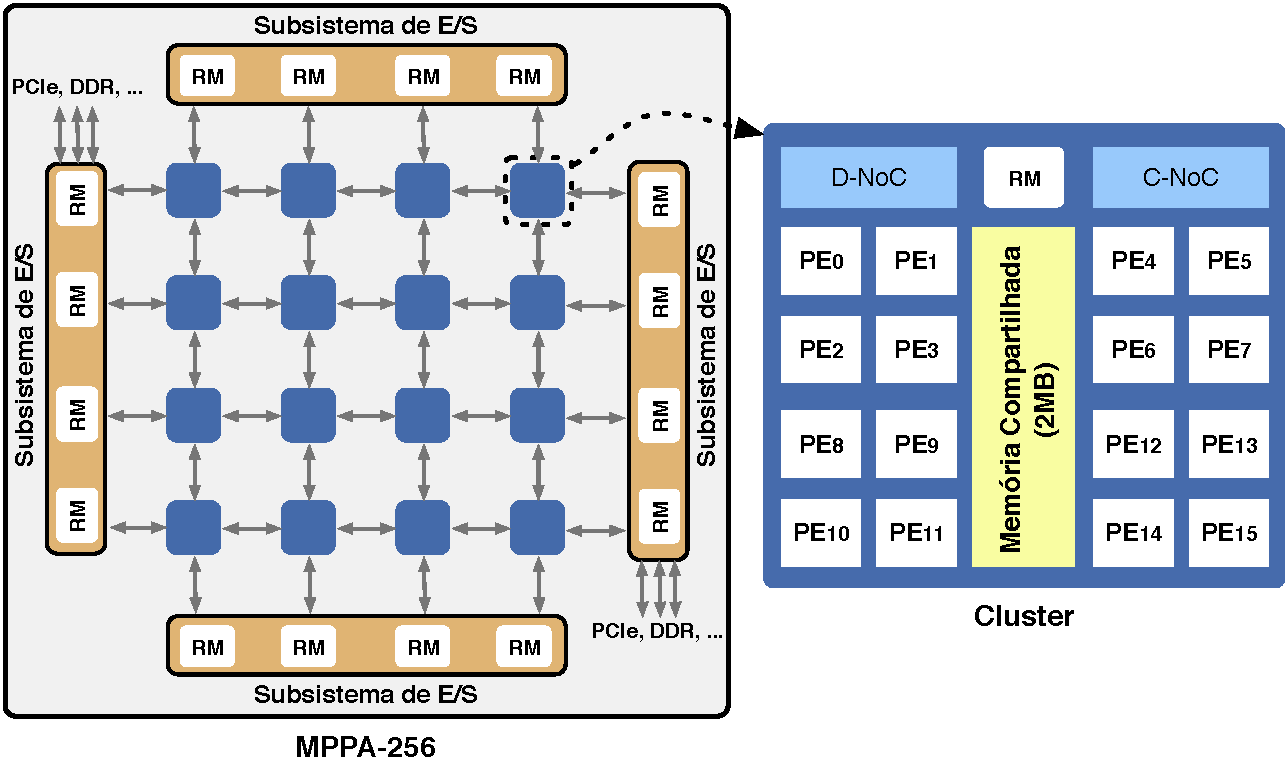
\includegraphics[width=0.75\textwidth]{figs/mppa-overview.pdf} \\
    \legend{Fonte: \cite{castro2013}}
    \label{fig:mppaOverall}
\end{figure}


Trabalhos anteriores mostraram que desenvolver aplicações paralelas otimizadas
para o \mppa é um grande desafio~\cite{francesquini:hal-01092325} devido a alguns
fatores importantes, tais como: o modelo de memória distribuída presente no
\mppa, a capacidade de memória dentro do \textit{chip} e a comunicação explícita
através da \noc. Mais detalhes sobre esses desafios são apresentados em
~\cite{wscad2017}.

\section{Esqueletos paralelos}
\label{sec:esqueletosparalelos}

Um esqueleto paralelo é responsável por abstrair um determinado padrão de computação paralela. Para utilizar um esqueleto o programador definirá as operações principais a serem realizadas, ou seja, definirá o \textit{kernel} da computação. E o esqueleto será responsável em compor essa função definida pelo usuário, devendo ser executada de maneira correta, paralela e o mais eficiente possível.

A abstração de padrões paralelos contribui para a simplificação e desenvolvimento, além de reduzir o custo de modelagem, facilitar a transformação e otimização das computações.

Devido ao alto nível de abstração, esqueletos paralelos possuem alta afinidade com conceitos presentes nas linguagens de programação, como \textit{templates} e \textit{generics} da linguagem de programação orientada a objetos, assim os esqueletos paralelos exploram estes mecanismos \cite{Gorlatch2011}.

\subsection{Padrão estêncil}
\label{subsec:stencil}

Dentre os padrões presentes na literatura, o padrão estêncil é muito utilizado devido a sua aplicação nos campos de simulações meteorológicas, comportamento de fluídos físicos, entre outros.

Ilustrado pela Figura~\ref{fig:stencil}, funciona da seguinte forma. Para cada elemento de uma estrutura $n$-dimensional é computado um novo valor relativo aos vizinhos do elemento atual. Os vizinhos de um elemento são determinados pela máscara da computação. Por fim, cada novo valor computado é atribuído à sua célula respectiva em uma estrutura $n$-dimensional de saída. Em aplicações estêncil iterativas, a estrutura de saída é utilizada como estrutura de entrada de uma nova iteração da aplicação.

\begin{figure}
    \centering
    \caption{O padrão estêncil.}
    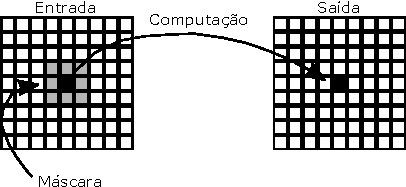
\includegraphics[width=0.75\textwidth]{figs/stencilComputation.pdf} \\
    \legend{Fonte: \cite{wscad2017}}
    \label{fig:stencil}
\end{figure}

\subsection{\pskel}

O \pskel é um \fw de programação em alto nível para aplicações baseadas no
padrão estêncil, baseado no conceito de esqueletos paralelos, oferecendo suporte para a execução dessas aplicações em
ambientes heterogêneos, incluindo \cpu e \gpu. \pskel oferece um interface única de programação, desacoplada do \textit{back-end} de execução, permitindo que o usuário se preocupe apenas em implementar o \textit{kernel} estêncil que descreve a computação, enquanto o \fw fica responsável pela tradução das abstrações descritas para código paralelo de baixo nível em C++, gestão de memória e transferência de dados, tudo isso de forma transparente para o usuário~\cite{CPE:CPE3479}.

\todo[inline]{Explicar o PSkel de maneira mais detalhada (classes, métodos, kernel, com pseudo-código como no artigo do euro-par). Note, por exemplo, que na tua proposta tu falas de \texttt{Array2D}. Se isso não for explicado aqui ninguém intenderá a proposta.}

\section{PSkel-MPPA}
\label{sec:pskel-mppa}

A adaptação PSkel-MPPA, é uma adaptação do \pskel proposta por~\cite{wscad2017}, ela faz uso de uma \api similar à POSIX \ipc para comunicação, e será tratada como \ipc no decorrer deste trabalho. Nela, são utilizados portais de comunicação para o envio de dados e o método de \textit{strides}  para gerenciar explicitamente o envio e recebimento de \textit{tiles}. Essa adaptação possibilita o uso do \fw PSkel com o processador \manycore \mppa.

\todo[inline]{O que são os portais? É importante explicar como a comunicação era feita na versão anterior. Com isso, tu terás a base para explicar como tu ``pretendes'' otimizar a comunicação usando a nova API. O que são os \textit{tiles}? Explique melhor a solução existente. Para isso, pegue o texto do Capítulo 4 e coloque aqui, adaptando-o quando necessário.}